%%%%%%%%%%%%%%%%%%%%%% DOKUMENT_HEADER %%%%%%%%%%%%%%%%%%%%%%%%%%%%%%%%%
\documentclass[a4paper, 10pt]{article}

%-------------------------- Packete ------------------------------------
\usepackage[english]{babel}
\usepackage{graphicx}
%\usepackage{a4wide}        % seiten mehr ausf�llen
\usepackage{amsfonts}
\usepackage{amsmath}
\usepackage{amssymb}
\usepackage{fancyhdr}
\usepackage{color}
\usepackage[colorlinks=false,linkbordercolor=0 0 0]{hyperref}
\usepackage{tikz}
\usepackage{algorithmic}
\usepackage{algorithm}
\usepackage{fp}
%\usepackage[pdftex,pdfstartview=FitB,colorlinks=true,citecolor=black,
%urlcolor=black,linkcolor=blue,pdfpagemode=None]{hyperref}

\tikzstyle{normalnode}=[draw,%
                          rectangle,%
                          shade,%
                          minimum size  = 1.0cm,%
                          node distance = 1.3cm]
 \tikzstyle{normalnode2}=[draw,%
                          rectangle,%
                          shade,%
                          minimum size  = 1.0cm,%
                          node distance = 1.0cm]
  \tikzstyle{start}=[draw,fill=green!70,rectangle, minimum size=1.0cm,node distance=1.3cm]                        
  \tikzstyle{goal}=[draw,fill=red!70,rectangle, minimum size=1.0cm,node distance=1.3cm]
  \tikzstyle{goal2}=[draw,fill=red!70,rectangle, minimum size=1.0cm,node distance=1.0cm]
  \tikzstyle{agent}=[draw,fill=blue!70,circle,minimum size=0.6cm]
  \tikzstyle{dummy}=[circle]


%------------------------- Einstellungen -------------------------------
\setlength\parskip{\medskipamount}
\setlength\parindent{0pt}

%================== Kopfzeilenlayout ====================
\pagestyle{fancy}
%\renewcommand{\chaptermark}[1]{\markboth{\chaptername\ \thechapter.\ #1}{}}
%\renewcommand{\sectionmark}[1]{\markright{\thesection\ #1}{}}
\fancyhf{}
\fancyhead[LE,RO]{\thepage}
\fancyhead[RE]{\sffamily \rightmark}
\fancyhead[LO]{\sffamily \leftmark}
\fancyfoot{\sffamily}
\pagestyle{fancy}

%_-------------------------Definitionen---------------------------------
\newcommand{\FO}{\textrm{FO}}      % romanstyle FO
\newcommand{\cL}{\mathcal{L}}      % kalligraphisches L
\newcommand{\cC}{\mathcal{C}}      % kalligraphisches C
\newcommand{\N}{\mathbb{N}}        % nat�rliche Zahlen N
\newcommand{\gdw}{\Leftrightarrow} % genau dann wenn \gdw
\newcommand{\folgt}{\Rightarrow}   % \folgt f�r daraus folgt Pfeil
% \eodef \eobew
% Liefert einen rechtsbuendigen Kasten zur Kennzeichnung des Endes einer 
% Definition (leer) und eines Beweises (ausgefuellt).
\newcommand{\eobew}{\par\begin{flushright}$\square$\end{flushright}}
\newcommand{\eodef}{\begin{flushright}$\blacksquare$\end{flushright}}
\newcommand{\argmax}[1]{\underset{#1}{\operatorname{argmax}}\;}
\newcommand{\argmin}[1]{\underset{#1}{\operatorname{argmax}}\;} 
\DeclareMathOperator*{\argmin}{argmin}
\DeclareMathOperator*{\argmax}{argmax}

%%%%%%%%%%%%%%%%%%%%%%%%%%%%%%% DOKUMENT %%%%%%%%%%%%%%%%%%%%%%%%%%%%%%%
\begin{document}

%%%%%%%%%%%%%%%%%%%%%%%%%%%%%% TITELSEITE %%%%%%%%%%%%%%%%%%%%%%%%%%%%%%
 \begin{titlepage}
     \begin{center}
       \large
       \textsc{Rheinisch-Westf\"alische Technische Hochschule Aachen}\\
       Knowledge-Based Systems Group \\
       Prof. G. Lakemeyer, Ph.D. \\ 
       \vspace{3 cm}
       \huge Seminar Foundations of AI\\
       \large summer term 2009 \\
       \vspace{1 cm}
       \huge
       Reinforcement Learning\\
       \vspace{4 cm}
       \Large Christian Kalla\\
       \vspace{3 cm}
       last build: \today \\
     \end{center}
 \end{titlepage}

%\title{Multi-agent Reinforcement Learning}
%\date{\today}
%\author{Christian Kalla}
%\maketitle

%\clearpage
%% %%%%%%%%%%%%%%%%%%%%%%% INHALTSVERZEICHNIS %%%%%%%%%%%%%%%%%%%%%%%%%%
\tableofcontents
\clearpage

%% %%%%%%%%%%%%%%%%%%%%%%%%%%%%%%%%%%%%%%%%%%%%%%%%%%%%%%%%%%%%%%%%%%%%%
\section{Introduction}
\label{sec:intro}
Reinforcement Learning can be regarded as one of the most natural ways of learning by interacting with the environment.\\
In contrast to other methods of machine learning, an agent only learns by receiving feedback from its environment and trying out which actions yield the highest return in a certain situation. It does not seem astonishing at all that one of the roots of this method of learning can be found in psychology. An illustrative example is comparing this method to the way infants learn when making their first steps in an unknown environment. For example crying will often lead to the result that the parents get something to drink or to eat for the child, which can be regarded as a reward. So crying would be learned as a good action when trying to reach the goal of getting food.  Another analogy is the situation when learning to drive (also referred to in \cite{Markelic04reinforcementlearning}). Neglecting the driving instructor who could turn this example into one for supervised learning, driving can also be learned by paying attention to the reactions of the environment (e.g. the car and other road users). One goal could be to get no bad reaction of the other drivers, so honking could be a bad signal from the environment and remind you to drive faster for example. More of those analogies can be found in \cite{Sutton98}.\\
One important fact is that the aim of an agent is always to maximize the sum of rewards on the way to its goal and not to focus on single rewards. This stresses the need of a so called value function that tells the agent how good certain states are with respect to the expected sum of rewards.\\
The first section of this paper will deal with methods and algorithms to compute this value function and point out the occuring difficulties and will conclude with an overview of some interesting applications. In this context Markov Decision Processes (see \cite{Barto90learningand},\cite{Howard60}) play an important role which assume a stationary environment that does not contain other adaptive agents. The arising problem from this is that cooperation of agents that would be important for many multiplayer games cannot be considered as it is not supported by the mathematical framework.\\
This problem is regarded in the second section of this paper mainly considering the work of \cite{Littman94}. Here Markov Games which explicitely support multi-agent environments are used to adapt the Q-Learning algorithm presented in the first section to develop an agent for a simple version of soccer. The corresponding algorithm will be presented and the results against other agents will be shown and discussed.

%% %%%%%%%%%%%%%%%%%%%%%%%%%%%%%%%%%%%%%%%%%%%%%%%%%%%%%%

\section{Reinforcement learning in general}
\subsection{The main idea behind reinforcement learning}
The general idea of reinforcement learning is visualized in figure \ref{agentWorldModel}. An agent starts at time $t$ in a given situation $s_{t}$ and chooses an action $a_{t}$. This action takes him to a new state $s_{t+1}$ and gives a reward $r_{t+1}$ as feedback. The new state and the reward depend on the dynamics of the environment and may be deterministic or stoachastic. This means that the rewards and successor states are either clearly defined (e.g. in games like chess) or occur with a certain probability (this could be the case in real-time environments). In many scenarios the reward is often not given directly, but when reaching the goal. This often leads to the problem that an agent does not know how good his actions were before having reached the goal state for the first time.
\begin{figure}
\centering
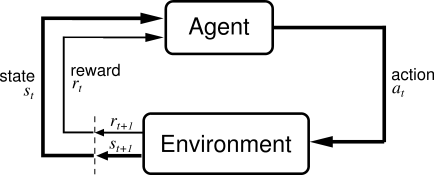
\includegraphics[scale=0.5]{pics/worldModel.png}
\caption{The model of the agent and its environment for reinforcement learning (taken from \cite{Sutton98})}
\label{agentWorldModel}
\end{figure}
\subsection{Important problems}
\paragraph{The control problem}
\paragraph{Problem of exploration and exploitation}
A difficult task for an agent in an environment is to find the right balance between using the information gained by already visited states (e.g. the values of states in the reinforcement learning case) and trying to explore the environment by taking actions leading to unknown states. One problem that can occur during reinforcement learning is that once the agent has found a way to the goal, it will always use the same way again, without knowing if there is another (probably better) one. We all know this problem when driving to work for example being annoyed about traffic jams, for example. Of course one way found by our initial policy (e.g. the motorway) definitely leads to the goal, but having driven the same way for many times, we try out something new the next day and "explore" the state space in some way. Of course this may also lead to worse results than before, but there also might be faster ways (analogous to better policies) leading to the goal. $\epsilon$-greedy policies are an example for policies that in general choose the action leading to the state with the highest value, but sometimes (with probability $\epsilon$) take random actions.
\paragraph{The prediction problem}
\paragraph{Partial observability problem}
\paragraph{Curse of Dimensionality}
difficulty to determine optimal state and action sets
\paragraph{Credit Structuring Problem}
\subsection{Value function and Policies}
As mentioned before, the main goal of an agent is to find an optimal policy $\pi^{*}$, i.e. a roadmap that enables the agent to choose the right action in each state in order to reach its goal as fast as possible. Or more formally:
\newtheorem {definition} {Definition}
\begin{definition}[Policy]
Let $S$ be a set of states and $A$ be a set of actions an agent can choose in its environment.\\
A mapping $\pi:S \rightarrow A \ \forall s \in S$ is called a policy .
\end{definition}
\begin{definition}[Optimal Policy]
A policy $\pi^{*} \in \Pi$ ($\Pi$ denotes the set of all possible policies) that maximizes the quantity
\begin{equation}
R=r_{0}+r_{1}+...+r_{n}
\end{equation}
for Markov decesion processes with a terminal state or the quantity
\begin{equation}
R=\sum_{t}{\gamma^{t}r_{t}}
\end{equation}
for MDPs without a terminal state ($0 \leq \gamma \leq 1$ denotes the discounting factor) is called optimal policy.
\end{definition}
In order to find optimal policies, a function that defines the value of a state itself (V-function) or the value for choosing an action in a given state (Q-function) is needed. As the goodness of a state always depends on the expected future reward, it depends also on the future actions taken by the agent. That is why value functions always have to be considered with respect to a certain policy (denoted by the index $\pi$). More formally:
\begin{definition}[State-value function]
The function
\begin{equation}
V^{\pi}(s)=E_{\pi}\left\{R_{t}|s_{t}=s \right\}=E_{\pi}\left\{ \left. \sum_{k=0}^{\infty}{\gamma^{k}r_{t+k+1}}\right|s_{t}=s  \right\}
\end{equation}
is called the state-value function for policy $\pi$. $E_{\pi}{}$ denotes the expected value given the fact that the agent follows the policy $\pi$ with an arbitrary time step $t$.
\end{definition}
The action-value function $Q^{\pi}(s,a)$ that assigns values to a state-action pair is defined similarly:
\begin{definition}[Action-value function]
The function
\begin{equation}
Q^{\pi}(s,a)=E_{\pi}\left\{R_{t}|s_{t}=s, a_{t}=a \right\}=E_{\pi}\left\{ \left. \sum_{k=0}^{\infty}{\gamma^{k}r_{t+k+1}}\right|s_{t}=s, a_{t}=a  \right\}
\end{equation}
is called the action-value function for policy $\pi$. 
\end{definition}
As the goal of reinforcement learning is to find an optimal policy from the initial state to the goal, there have to be methods to compute an optimal policy efficiently. A naive way to do so would be trying out all possible policies which means taking every possible action in every state and receiving the rewards from the environment. Of course the complexity of this approach would be too high, because the set of states and the set of actions are very large in general, so exploring the whole search space is inefficient. There are many methods to approximate optimal value functions and therefore also give an approximation for an optimal policy. The first two methods that will be presented use dynamic programming and perform policy or value iteration. This means to start with an arbitrary policy for example, determine the resulting value function for this policy and use this value function to get an improved policy. After this the same procedure is iterated several times until the optimal policy is found (or at least a good approximation). A significant disadvantage of those dynamic programming methods is that they require a complete model of the environment and so they are not applicable if the environment is unknown to the agent.\\
In contrast Monte-Carlo methods do not require this model. Here the value function is learned by averaging the rewards of many episodes. Because the transition probabilities of the environment are not known (in contrast to DP methods), they have to be determined by many iterations.\\
Another important kind of reinforcement learning algorithms do not require this environment model and use Temporal Difference learning. This means that they compute the difference between the two values of a value function at different time points (e.g. $Q(s,a)-Q(s',a')$). The presented algorithms Q-learning and SARSA are two examples for this kind of learning method.
\subsection{Separation from other machine learning approaches}
This section gives a brief overview of the placement of reinforcement learning in machine learning.
Machine learning in general distinguishes between three learning approaches: Supervised learning, unsupervised learning and reinforcement learning. The main task of all those approaches is to use the knowledge gained from previous experience to solve new tasks using this knowledge.\\
In supervised learning the agent is given a set of examples containing input and the correct output. After that the agent adapts the parameters of its model (e.g. the parameters of a probability distribution) in such a way that the seen data is represented best. This is often done by the maximum likelihood method. One example for this kind of learning could be the recognition of handwritten letters or digits, where the agents gets some example images with the correct letter or digit. After that the model is used to classify some unknown input text.\\
In unsupervised learning the agent is just given the data itself, but not the correct class, so there is no "teacher" as in supervised learning. In order to learn from the data and derive a model, clustering methods and the EM algorithm play an important role.\\
Reinforcement learning differs from both previous approaches, because the agent has to discover its environemnt on its own, without having a supervisor that tells him the correct actions. The only feedback if the chosen action was good or bad can be extracted from the reward or punishment the action brings.\\
But which advantages does this approach have?  In \cite{Sutton98} an example of a Tic-Tac-Toe playing agent is given. Everybody knows that this game always ends up with a draw when both players make the best moves, but it could also be the case that the opponent agent shows weaknesses in certain positions, although it might play well otherwise. A standard approach to those kinds of zero sum games is applying the Minimax algorithm with a simple heuristic that guarantees to gain the best result assuming that the opponent always chooses the best move. One disadvantage here is that always optimal play of the opponent is assumed, although this might be wrong. Applying reinforcement learning algorithms to this kind of game would result in an agent that discovers the weaknesses of its opponent and exploits, whereas a minimax approach would just be able to reach a draw for example. A quite strong agent for the game of backgammon using reinforcement learning techniques is presented at the end of the first section.
\subsection{The Markov Property and Markov Decision Processes}
The goal of reinforcement learning is to maximize an agents reward and to find an optimal policy leading to a goal state. But how do environments behave, if an agent chooses an action in a state at a given time? The first thing we have to consider when answering this question is to imagine different environments and think about their characteristics. At this point we have to distinguish between deterministic and stochastic environments. Playing chess is an example for a deterministic environment. There is a specified choice of actions in each state and each of those actions leads to a clearly defined next state. The environment we live in does not necessarily lead to one defined state when taking an action. Instead an action could lead to several states and each of those successor states can occur with a given probability. For example the state "Driving drunk" with the action "Driving in an erratic manner" could lead to the state "Getting stopped by the police", but also to the state "Arriving safe at home". Another important question is if the probability of the successor states depends on the actions taken before, or if just the current state counts for future decisions. This is exactly what the Markov Property demands. For the chess example this question is easy to answer: The agent has to make his decision based on the current position (i.e. the current state) and the environment also does not care about what happened in the past. For other kinds of environment this conditional independence from earlier states cannot be guaranteed in many cases. One thing that might be confusing in this context is the definition of a state itself. The definition of a state takes information about the agents' sensors as input, so a state can depend from sensations made somewhen earlier. The Markov expression can formally be expressed as follows:
\begin{equation}
\begin{align}
&Pr\left\{s_{t+1}=s',r_{t+1}=r|s_{t},a_{t},r_{t},s_{t-1},a_{t-1},...,r_{1},s_{0},a_{0}\right\}\\
=&Pr\left\{s_{t+1}=s',r_{t+1}=r|s_{t},a_{t}\right\}
\end{align}
\end{equation}
Every reinforcement learning task whose states have the Markov Property is called a Markov Decision Process (MDP). If the state and action space are finite we talk about finite MDPs. MDPs are formally defined in \cite{Howard60} and consist of the following components:
\begin{itemize}
\item a set of states $\mathcal{S}$
\item a set of actions $\mathcal{A}$
\item a set of rewards $\mathfrak{R}$
\item a transition function $T:\mathcal{S}\times \mathcal{A}\rightarrow PD(\mathcal{S})$ where $PD(\mathcal{S})$ denotes the set of probability distribution over $\mathcal{S}$
\item a reward function $R:\mathcal{S} \times \mathcal{A} \rightarrow \mathfrak{R}$
\end{itemize}
In stochastic environments the successor state is not only defined by an action, but also by a probability distribution defining the transition probabilities:\\
\begin{equation}
\mathcal{P}_{ss'}^{a}=Pr \left\{s_{t+1}=s'|s_{t}=s,a_{t}=a \right\}
\end{equation}
Accordingly the expected value of the next reward can be defined as
\begin{equation}
\mathcal{R}_{ss'}^{a}=E \left\{r_{t+1}|s_{t}=s,a_{t}=a,s_{t+1}=s' \right\}
\end{equation}
\subsection{How to find optimal policies?}
Gives an overview of algorithms to compute optimal policies.
\subsubsection{Dynamic Programming}
The most obvious way of finding an optimal policy is using dynamic programming techniques. One way is to start with an arbitrary policy, derive the value function and improve the policy thereafter (policy iteration). Another way is to start with an initial value for all states and adapt this value function iteratively (value iteration).
\paragraph{Value iteration}
\paragraph{Policy Iteration}
An illustration of the principle of policy iteration can be found in the following figure taken from \cite{Sutton98}.
\begin{figure}
\fbox{
\begin{equation*}
\pi_{0}\stackrel{evaluation}{\longrightarrow}V^{\pi_{0}} \stackrel{improvement}{\longrightarrow}{\pi_{1}} \stackrel{evaluation}{\longrightarrow}{V^{\pi_{1}}}... \stackrel{improvement}{\longrightarrow} \pi_{*} \stackrel{evaluation}{\longrightarrow}{V^{\pi_{*}}}
\end{equation}
}
\caption{The principle of policy iteration}
\end{figure}
The algorithm in pseudocode is given in \ref{alg1}.
\begin{algorithm}[tb]
\caption{Policy Iteration}
\label{alg1}
\begin{enumerate}
\item \textbf{Initialization}
\begin{algorithmic}
\STATE $V(s) \in \mathfrak{R}$ and $\pi(s) \in \mathcal{A}$ arbitrarily for all $s \in \mathcal{S}$
\end{algorithmic}
\item \textbf{Policy Evaluation}
\begin{algorithmic}
\REPEAT
\STATE $\delta \gets 0$
\FOR {$s \in \mathcal{S}$}
\STATE $v \gets V(s)$
\STATE $V(s) \gets \sum_{s'}{\mathcal{P}_{ss'}^{\pi(s)}(\mathcal{R}_{ss'}^{\pi(s)}+\gamma V(s'))}$
\STATE $\delta \gets \max(\delta,|v-V(s)|)$
\ENDFOR
\UNTIL{$\delta < \theta$ (a small threshold to be reached)}
\end{algorithmic}
\item \textbf{Policy Improvement}
\begin{algorithmic}
\STATE $policy-stable \gets true$
\FOR {$s \in \mathcal{S}$}
\STATE $b \gets \pi(s)$
\STATE $\pi(s) \gets \arg\max_{a}{ \sum_{s'}{\mathcal{P}_{ss'}^{a}(\mathcal{R}_{ss'}^{a}+\gamma V(s'))}}$
\IF{$b \neq \pi(s)$}
\STATE $policy-stable \gets false$
\ENDIF
\ENDFOR
\IF{$policy-stable$}
\STATE STOP
\ELSE GOTO 2.
\ENDIF
\end{algorithmic}
\end{enumerate}
\end{algorithm}
The example in figure \ref{vla} underlines how the presented algorithm works. The task of the agent is to get from its starting state (the green square) to the goal (the red square) by moving up, down, left and right. The agent only receives a reward if the goal state is reached (+100), otherwise it does not gain anything (0). The initial policy is deterministic and seems to be quite stupid, but according to the algorithm the agent improves this policy quite fast. The discount factor $\gamma$ is set to $0.9$.
\begin{figure}[tb]
\begin{minipage}[t]{0.475 \textwidth}
\begin{center}
  \begin{tikzpicture}
            \node[start] (a)  {0};
            \node[normalnode][right of=a]  (b) {0};
            \node[goal][right of=b]  (c) {};
            \node[normalnode][below of=a]  (d) {0};
            \node[normalnode][right of=d]  (e) {0};
            \node[normalnode][right of=e] (f) {0};
            \draw [->] (a.south) to  node[right] {\tiny 0}  (d.north);
            \draw [->] (d.east) to node[above] {\tiny 0} (e.west);
            \draw [->] (e.north) to node[right] {\tiny 0} (b.south);
            \draw [->] (b.east) to node[above] {\tiny 100} (c.west);
            \draw [->] (f.west) to node[above] {\tiny 0} (e.east);	
  \end{tikzpicture}
\caption{Initial situation of the grid world with rewards for the actions}
\end{center}
\end{minipage}
\begin{minipage}[t]{0.475 \textwidth}
\begin{center}
 \begin{tikzpicture}
            \node[start] (a)  {0};
            \node[normalnode][right of=a]  (b) {100};
            \node[goal][right of=b]  (c) {};
            \node[normalnode][below of=a]  (d) {0};
            \node[normalnode][right of=d]  (e) {0};
            \node[normalnode][right of=e] (f) {0};
            \draw [->] (a.south) -- (d.north);
            \draw [->] (d.east) -- (e.west);
            \draw [->] (e.north) -- (b.south);
            \draw [->] (b.east) -- (c.west);
            \draw [->] (f.west) -- (e.east);	
  \end{tikzpicture}
\caption{situation after one value update}
\end{center}
\end{minipage}
\begin{minipage}[t]{0.475 \textwidth}
\begin{center}
  \begin{tikzpicture}
            \node[start] (a)  {72,9};
            \node[normalnode][right of=a]  (b) {100};
            \node[goal][right of=b]  (c) {};
            \node[normalnode][below of=a]  (d) {81};
            \node[normalnode][right of=d]  (e) {90};
            \node[normalnode][right of=e] (f) {81};
            \draw [->] (a.south) -- (d.north);
            \draw [->] (d.east) -- (e.west);
            \draw [->] (e.north) -- (b.south);
            \draw [->] (b.east) -- (c.west);
            \draw [->] (f.west) -- (e.east);	
  \end{tikzpicture}
\caption{situation after all value updates}
\end{center}
\end{minipage}
\begin{minipage}[t]{0.475 \textwidth}
\begin{center}
  \begin{tikzpicture}
            \node[start] (a)  {72,9};
            \node[normalnode][right of=a]  (b) {100};
            \node[goal][right of=b]  (c) {};
            \node[normalnode][below of=a]  (d) {81};
            \node[normalnode][right of=d]  (e) {90};
            \node[normalnode][right of=e] (f) {81};
            \draw [->] (a.east) -- (b.west);
            \draw [->] (d.east) -- (e.west);
            \draw [->] (e.north) -- (b.south);
            \draw [->] (b.east) -- (c.west);
            \draw [->] (f.north) -- (c.south);	
  \end{tikzpicture}
\caption{situation after policy change}
\end{center}
\end{minipage}
\begin{minipage}[t]{0.475 \textwidth}
\begin{center}
  \begin{tikzpicture}
            \node[start] (a)  {81};
            \node[normalnode][right of=a]  (b) {100};
            \node[goal][right of=b]  (c) {};
            \node[normalnode][below of=a]  (d) {81};
            \node[normalnode][right of=d]  (e) {90};
            \node[normalnode][right of=e] (f) {100};
            \draw [->] (a.east) -- (b.west);
            \draw [->] (d.east) -- (e.west);
            \draw [->] (e.north) -- (b.south);
            \draw [->] (b.east) -- (c.west);
            \draw [->] (f.north) -- (c.south);	
  \end{tikzpicture}
\caption{algorithm terminates after final value update}
\end{center}
\end{minipage}
\end{figure}
\subsubsection{Monte Carlo Methods}
The previously discussed dynamic programming methods had the clear disadvantage that they required a model of the dynamics of the environments, i.e. that the transition probabilities of each state-action pair had to be known in advance. Monte Carlo methods do not need this kind of knowledge. Instead they learn the value function of a state by computing the average return after the occurrence of a state generating a large number of episodes. If the number of generated episodes is high enough, the computed state value or state-action value will converge to the real one. Algorithm \ref{monteCarlo} shows a simple way of computing an optimal policy by generating an episode first and adapting the state-action value and the policy afterwards.\\
One important fact about Monte Carlo algorithms is that they do not make use of bootstrapping, i.e. they do not update the value of a state based on the values of successor states (also known as bootstrapping), but they compute the accumulated reward for each episode after the first occurrence of the state (or the state-action pair). This also makes them less "vulnerable" against environments that do not fulfill the Markov property.
\begin{algorithm}[tb]
\caption{Monte Carlo Algorithm for finding an optimal policy}
\label{monteCarlo}
\begin{algorithmic}
\STATE Initialize $\forall s \in \mathcal{S},a \in \mathcal{A}(s)$:
\STATE $Q(s,a) \gets arbitrary$
\STATE $\pi(s) \gets arbitrary$
\STATE $Returns(s,a) \gets empty list$
\REPEAT
\STATE Generate an episode using policy $\pi$ and a random starting state
\FORALL{pairs $(s,a)$ appearing in the generated episode}
\STATE $R \gets$ return following the first occurence of $(s,a)$
\STATE Append $R$ to $Returns(s,a)$
\STATE $Q(s,a)\gets average(Returns(s,a))$
\ENDFOR
\FORALL{states $s$ in the episode}
\STATE $\pi(s)=\arg\max_{a}{Q(s,a)}$
\ENDFOR
\UNTIL{final number of episodes is reached}
\end{algorithmic}
\end{algorithm}
\subsubsection{Temporal Difference Learning}
Algorithms that make use of temporal difference learning perform bootstrapping (as dynamic programming methods do), but do not need a model of the environment (a property that also applies to Monte Carlo methods). The term "temporal difference" just means that the value update of a state depends on the value of another state at a different timepoint (namely the successor state). In connection to this kind of learning methods the terms "on policy" and "off policy" are often used. "On policy" means that the policy that is used to generate an episode (the behaviour policy) is the same as the policy that is evaluated and improved (the estimation policy). In "off policy" methods those two policies can be independent. The advantage of this is that the state space could be explored better than in an "on policy" method, because episodes generated by a random policy ensure that not only similar episodes are generated (as it could be the case if a greedy policy is used both for estimation and behaviour control). Today TD-learning algorithms are very often applied for reinforcement learning problems.
\paragraph{The Q-Learning algorithm}
The Q-Learning algorithm is an off-policy control algorithm introduced in 1989 by C.J.C.H. Watkins and was quite a breakthrough at this time. It approximates the optimal state-action function $Q^{*}$ independent of the policy being followed. the Q-learning algorithm (in pseudocode) can be found in algorithm \ref{qlearning}. The basic idea is to generate a state-action pair by the behaviour policy and to update the value of the old state-action pair by observing the reward and the value of the highest state-action pair of the folowing state after executing the one generated by the policy. Of course again the discount factor $\gamma$ and the learning rate, denoted by $\alpha$ play a role. As already mentioned, the Q-Learning algorithms plays an important role in reinforcement learning, because it is widely used and part of many applications. One example is the backgammon-playing agent by Tesauro.
\begin{algorithm}[tb]
\label{qlearning}
\caption{Q-Learning algorithm}
\begin{algorithmic}
\STATE Initialize $Q(s,a)$ arbitrarily
\FOR{each episode}
\STATE Initialize $s$
\REPEAT
\STATE Choose a from s using policy derived from $Q$
\STATE Take action a and observe $a,s'$
\STATE $Q(s,a) \gets Q(s,a)+\alpha(r+\gamma \max_{a'} Q(s',a') - Q(s,a))$
\STATE $s \gets s'$
\UNTIL{s is terminal}
\ENDFOR
\end{algorithmic}
\end{algorithm}
\paragraph{Sarsa}
This algorithm was invented by Rummery and Niranjan in 1994 and is also regarded as a popular algorithm for reinforcement learning. In contrast to the Q-Learning algorithm it is an on policy approach and makes use of the following update rule:
\begin{equation}
Q(s_{t},a_{t}) \gets Q(s_{t},a_{t})+\alpha(r_{t+1}+\gamma Q(s_{t+1},a_{t+1})-Q(s_{t},a_{t})
\end{equation}
The basic idea of this update rule is to start with an inital state, choose an action according to the policy (note that the policy that chooses actions and the policy that is improved are identical), execute this action and receive the reward. Afterwards the best action according to the policy ($a_{t+1}$) is chosen and the Q-value of the old state action pair $Q(s_{t},a_{t})$ is updated. Then the procedure is repeated with the new state ($s_{t+1}$) and the new action ($a_{t+1}$) until a terminal state is reached. The complete algorithm is omitted at this point, but with the update rule as its central component it should not be hard to imagine how it should look like. The name of the algorithm "Sarsa" can be formed from the quintuple ($s_{t},a_{t},r_{t+1},s_{t+1},a_{t+1}$). A pseudocode example can be found in \cite{Sutton98}.
\paragraph{TD($\lambda$)}
\subsubsection{Eigibility traces as an improvement of reinforcement learning algorithms}
\subsection{Applications of reinforcement learning}
Gives an overview of some interesting applications of reinforcement learning. Perhaps some other interesting stuff could be added here.
\subsubsection{TD-Gammon}


\section{Multi-agent reinforcement learning}
As we have seen in the previous section, the term reinforcement learning is strongly related to Markov decision processes. Unfortunately the underlying mathematical framework for MDPs only supports environments with one agent. But how to apply the algorithms for MDPs to multiagent environments? Littman's paper (\cite{Littman94}) on multi-agent reinforcement learning addresses this problem and presents a variation of the Q-Learning algorithm, called "Minimax Q-Learning" based on Markov games.
\subsection{The framework of Markov Games}
Markov games are also called stochastic games and are formally defined as follows (also see \cite{owen95}):
\begin{definition}
A Markov game is defined by a set of states $\mathcal{S}$ and a collection of action sets $A_{1},...,A_{k}$ for each agent in the environment. A transition function $T$ maps a tuple of the current state and actions taken by each agent to a new state with a certain probability:
\begin{equation}
T:S \times A_{1} \times ... \times A_{k} \mapsto PD(\mathcal{S})
\end{equation}
Furthermore there are reward functions $R_{i}$ for each agent $i$:
\begin{equation}
R_{i}:S \times A_{1} \times ... \times A_{k} \mapsto \mathfrak{R}
\end{equation}
The aim of each agent $i$ is to maximize the expected sum of discounted rewards:
\begin{equation}
E\left\{\sum_{j=0}^{\infty}{\gamma^{j} r_{i,t+j}}\right\}
\end{equation}
\end{definition}
As the mathematics of those multiplayer games can get very complicated, Littman simplifies it considering only two agents with opposed goals playing against each other. This assumption makes it possible to use a single rewards function that is maximized by the first agent and minimized by the second one. Nevertheless cooperation between agents can no longer be considered. This simplified game can be seen as a "Zero-sum markov game", because the sum of rewards of the agents is zero. One important thing to realize is that Markov games are a generalization of MDPs, in which the number of the opponents's actions (denoted by $|O|$) is 1.
\subsubsection{Finding optimal policies in Markov games}
There are some important differences between optimal policies in markov games and markov decision processes. The aim of an agent in an MDP is to maximize the sum of discounted rewards. The same applies to Markov games, but here it can not be assured that there is an undominated policy. That means for every policy it could be the case that there is a state from which another policy would return a higher sum of discounted rewards than the current one. So in contrast to Markov games, each MDP has an undominated optimal deterministic policy which is also stationary (i.e. it does not depend on the time). As optimality of a policy in Markov games always depends on the behaviour of the opponent, an optimal policy is defined as a policy that assures the highest reward assuming optimal play of the opponent. Taking this definition, also every Markov game has at least one optimal (and even stationary) policy. But the deciding difference between optimal policies in MDPs and those in Markov games is that the policies in Markov games may be stochastic, whereas it is guaranteed that there is an optimal deterministic policy in an MDP.\\
An easy example is the game of "rock-paper-scissors". It is not hard to realize that choosing one of the three symbols at random is a better policy than always taking the same symbol so that it could happen to be second guessed. Also the simplified version of soccer presented later on requires a stochastic policy in certain situations.\\
But how to find the optimal policy in Markov games?\\
Similar to MDPs we can define $V(s)$ as the expected reward for the optimal policy in state s and $Q(s,a,o)$ as the expected reward when taking action $a$ in state $o$ knowing that the opponent has chosen action $o$. According to MDPs the value of a state can be expressed as
\begin{equation}
V(s)=\max_{\pi \in PD(A)} \min_{o \in O} \sum_{a \in A}{Q(s,a,o) \pi_{a}}
\end{equation}
and the value of a state-action pair against the opponent action $o$ as
\begin{equation}
Q(s,a,o)=R(s,a,o)+\gamma \sum_{s'}{T(s,a,o,s')V(s')}
\end{equation}
Those equations look very similar to the equations for MDPs with the min and max operators and the opponent action as third tuple element as the only differences. The value function of a state $s$ can be computed by solving a so called "Matrix game" (a markov game with just one state and a matrix of rewards such as rock-paper-scissors) using linear programming techniques. Another way of getting optimal Q-values and therefore an optimal policy is transforming the Q-Learning algorithm mentioned in the first section of this paper to a similar algorithm for Markov games. The only change that has to be made to get this new algorithm is replacing the max operator in the update step of the Q-Learning algorithm with a minimax operator.
\subsection{The Minimax-Q learning algorithm}
The algorithm defined in Michael Littmans's paper (\cite{Littman94})

\begin{algorithm}[tb]
\caption{The Minimax-Q algorithm (adapted from \cite{Litman94})}
\begin{enumerate}
\item \textbf{Initialization}
\begin{algorithmic}
\STATE $\forall s \in \mathcal{S},a \in \mathcal{A}, o \in \mathcal{O}$
\STATE $Q(s,a,o) \gets 1$
\STATE $\forall s \in \mathcal{S}$
\STATE $V(s) \gets 1$
\STATE $\forall s \in \mathcal{S}, a \in \mathcal{A}$
\STATE $\pi(s,a) \gets 1/|A|$
\STATE $\alpha \gets 1.0$
\end{algorithmic}
\item \textbf{Choice of the action}
\begin{algorithmic}
\STATE return a random action with probability $explor$
\STATE Ohterwise:
\IF{current state is s}
\STATE return an action a with probability $\pi(s,a)$
\ENDIF
\end{algorithmic}
\item \textbf{Learning phase}
\begin{algorithmic}
\STATE Receive reward $r(s,a,o,s')$ for moving from state $s$ to $s'$
\STATE $Q(s,a,o) \gets (1-\alpha) \cdot Q(s,a,o) + \alpha \cdot (rew+\gamma \cdot V(s'))$
\STATE Use linear programming to find $\pi(s,.)$ such that
\STATE $\pi(s,.) \gets \arg\max_{\pi'(s,.)}{\left\{\min_{o'}\left\{\sum_{a'}{\pi(s,a') \cdot Q(s,a',o')}\right\}\right\}}$
\STATE $V(s) \gets min_{o'}\left\{\sum_{a'}{\pi(s,a') \cdot Q(s,a',o')\right\}\right\}$
\STATE $\alpha \gets \alpha \cdot decay$
\end{algorithmic}
\end{enumerate}
\end{algorithm}

\subsection{Soccer as an application of the Minimax-Q algorithm}
\subsubsection{Game description and rules}
The game condidered in Littman's paper is a very simplified version of soccer. It is played between two agents A and B in a $4\times 5$ gridworld. Figure \ref{initialSetup} gives an overview of the initial setup of the grid. The red squares mark the goals and the aim of each agent is to step into one of those squares in order to score a goal. After a goal has been scored the game is reset to the initial state. Ball possession is assigned randomly to an agent at the beginning of the game. Unlike to normal soccer there is no real possibility to shoot, but you can just move with the ball or stand. So in each state an agent can choose between the actions $\mathcal{A}=\left\{N,S,E,W,stand\right\}$ where the first four actions stand for moving into a direction (north, south, east or west) and the last action (stand) keeps the situation unchanged. If an agent chooses an action that takes him to a square occupied by the other player, the player that did not move will get the ball. The game consists of rounds and the players select their moves at the same time without knowing the move of their opponent in advance. After the selection of the moves, they are executed in a random order.\\
The discount factor $\gamma$ is set to $0.9$ which assures that scoring goals earlier is better than scoring them later.\\
Figure \ref{probPolicyRequired} shows a situation that requires a probabilistic policy in order to win. Just suppose A always chooses to go left in this situation, then B would always choose the action stand and get the ball after both moves are executed. If A chooses a probabilistic policy, things look different. Now B does not know if a chooses "stand" or "south", because those actions are selected by a probabilistic policy and A could probably get a good opportunity to score (ore walk into) the opponent's goal.
\begin{figure}[tb]
\begin{minipage}[t]{0.475 \textwidth}
\begin{center}
\begin{tikzpicture}
\node[dummy] (01);
\foreach \i/\j in {0/1,1/2,2/3,3/4}
{
\node[normalnode2] [below of=\i1] (\j1) {};
	\foreach \x/\y in {1/2,2/3,3/4,4/5}
	{
		\node[normalnode2] [right of= \j\x] (\j\y) {};
		}
	}
\node[agent] (agentB) at (32) {B};
\node[agent] (agentA) at (24) {A};
\node[goal2] at (21);
\node[goal2] at (31);
\node[goal2] at (25);
\node[goal2] at (35);
\draw[->] (agentB) -- (32.north);
\draw[->] (agentB) -- (32.west);
\draw[->] (agentB) -- (32.east);
\draw[->] (agentB) -- (32.south);
\draw[->] (agentA) -- (24.north);
\draw[->] (agentA) -- (24.west);
\draw[->] (agentA) -- (24.east);
\draw[->] (agentA) -- (24.south);
\end{tikzpicture}
\caption{Initial situation}
\label{initialSetup}
\end{center}
\end{minipage}
\begin{minipage}[t]{0.475 \textwidth}
\begin{center}
\begin{tikzpicture}

\node[dummy] (01);
\foreach \i/\j in {0/1,1/2,2/3,3/4}
{
\node[normalnode2] [below of=\i1] (\j1) {};
	\foreach \x/\y in {1/2,2/3,3/4,4/5}
	{
		\node[normalnode2] [right of= \j\x] (\j\y) {};
		}
	}
\node[goal2] at (21);
\node[goal2] at (31);
\node[goal2] at (25);
\node[goal2] at (35);
\node[agent] (agentB) at (21) {B};
\node[agent] (agentA) at (22) {A};
\draw[->] (agentB) -- (21.north);
\draw[->] (agentB) -- (21.west);
\draw[->] (agentB) -- (21.east);
\draw[->] (agentB) -- (21.south);
\draw[->] (agentA) -- (22.north);
\draw[->] (agentA) -- (22.west);
\draw[->] (agentA) -- (22.east);
\draw[->] (agentA) -- (22.south);

\end{tikzpicture}
\caption{Situation that requires a probabilistic policy}
\label{probPolicyRequired}
\end{center}
\end{minipage}
\end{figure}
\subsubsection{Training and Testing}
\subsubsection{Results}
\begin{table}[htbp]
\caption{Results of games of the agents trained with different policies (taken from \cite{Littman94})}
\includegraphics[viewport=122 604 524 698,keepaspectratio,clip,page=6,scale=0.85]{../../ml94-final.pdf}
\end{table}

                                                                                

%\clearpage
%% %%%%%%%%%%%%%%%%%%%%%%%%%%%%%%%%%%%%%%%%%%%%%%%%%%%%%%%%%%%%%%%%%%%%%
\section{Related Work}
\label{sec:relatedwork}



%% %%%%%%%%%%%%%%%%%%%%%%%%%%%%%%%%%%%%%%%%%%%%%%%%%%%%%%%%%%%%%%%%%%%%%


%\clearpage
%% %%%%%%%%%%%%%%%%%%%%%%%%%%%%%%%%%%%%%%%%%%%%%%%%%%%%%%%%%%%%%%%%%%%%%


%%%%%%%%%%%%%%%%%%%%%%%%%%%%%%%%%%%%%%%%%%%%%%%%%%%%%%%%%%%%%%%%%%%%%%%%
%___________________ ABSCHNITT Ausblick __________________________
\section{Conclusion and Outlook}
\label{sec:conclusion_outlook}

Conclude with a summary and give an outlook on future stuff.

\clearpage
%% %%%%%%%%%%%%%%%%%%%%%%%%%%%%%%%%%%%%%%%%%%%%%%%%%%%%%%%%%%%%%%%%%%%%%
%\section{Bibliography}
%\label{sec:biblio}

\nocite{*}
\bibliographystyle{alpha}
\bibliography{sempaper}

%%%%%%%%%%%%%%%%%%%%%%%%%%%%%%%%%%%%%%%%%%%%%%%%%%%%%%%%%%%%%%%%%%%%%%%%
\end{document}

%% Emacs File Variables
%% Local Variables: %%
%% TeX-command-default: "pdflatex" %%
%% mode: LaTeX %%
%% End: %%
